\label{sec:toolingsoftware}
Für die Entwicklung der Firmware wurde das Zephyr Real-Time Operating System (RTOS) eingesetzt. Zephyr bietet eine modulare Architektur auf Basis von Device Trees. Dies ermöglicht eine gemeinsame Codebasis für alle Microcontroler und Peripheriegeräten. Darüber hinaus stellt das Framework eine Vielzahl vorgefertigter Treiber und Bibliotheken bereit, die für die vorliegende Arbeit unmittelbar nutzbar waren. Dazu zählen unter anderem Implementierungen für LoRaWAN, UART-gebundene GPS-Module, SD-Karten mit Dateisystemunterstützung, Displays (z.\,B. OLED beim ESP32-basierten Board) sowie Schnittstellen wie OneWire und I\textsuperscript{2}C für externe Sensoren. 

Die Implementierung der Firmware erfolgte in C++, da diese Sprache im Embedded-Bereich weit verbreitet ist und ebenso einer der 3 Hauptsprache, neben C und Rust, für Zephyr RTOS ist \autocite{LanguageSupportZephyr}. Auf zusätzliche externe Libraries wurde verzichtet, da die Funktionalität durch die Zephyr-Basis bereits vollständig abgedeckt war. \\

Das Software-Design folgt einem modularen Ansatz: Für jede Komponente existiert ein eigenständiges Modul, das während des Systemstarts initialisiert wird. Hierzu gehören insbesondere die SD-Karte, das GPS-Modul sowie beliebige Sensorschnittstellen. Alle implementierten externen Sensoren besitzen eine einheitliche \texttt{read()}-Methode, über die Messwerte ausgelesen werden können. Die Auswahl und Aktivierung einzelner Module erfolgt über die Projektkonfiguration in der Datei \texttt{prj.conf}. Auf diese Weise kann beispielsweise über den Eintrag:
\begin{verbatim}
lora_wan_tracker_temp_sensor=y
\end{verbatim}
die Einbindung eines Temperatursensors aktiviert werden. Dieser Ansatz ermöglicht eine flexible Anpassung der Firmware an unterschiedliche Anwendungsfälle, ohne tiefgreifende Änderungen am Quellcode vorzunehmen.

Ein Bestandteil des Software-Designs ist die Datenpaketstruktur, mit der die gesammelten Messwerte über LoRaWAN übertragen werden. Jedes Paket enthält zunächst die GPS-Daten und den Zeitstempel des Geräts in komprimierter Form. Hierzu werden Breiten- und Längengrad, Höhe, Genauigkeit sowie die Anzahl empfangener Satelliten als Big-Endian-Werte in ein Byte-Array codiert.

Im Anschluss an die GPS-Daten und Zeitdaten wird ein 4-Bit-Feld angefügt, das als Bitmap fungiert. Jedes Bit steht für einen spezifischen Sensor und zeigt an, ob für diesen Sensor Messwerte im aktuellen Paket enthalten sind. Die eigentlichen Sensordaten folgen in einer festgelegten Reihenfolge. Diese Struktur erlaubt eine flexible Erweiterung, da neue Sensortypen durch die Definition zusätzlicher Bits in der Bitmap ergänzt werden können, ohne die bestehende Protokollstruktur zu verändern. Eine Vollständige ansicht des Paketes kann Abbildung \ref{fig:lorawanPacket} entnommen werden.

\begin{figure}[H]
\centering
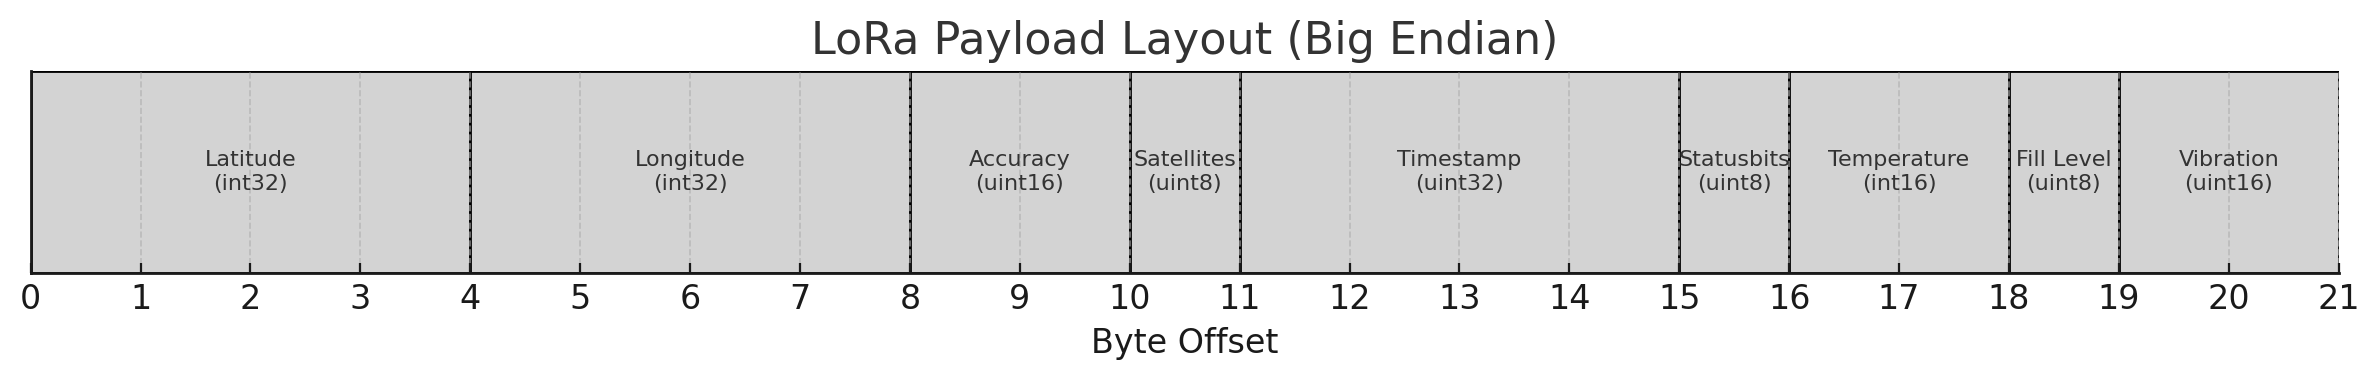
\includegraphics[scale=.5]{figures/asstes/lorawan-packet-layout.png}
\caption{Datensegment des LoraWAN Pakets}
\label{fig:lorawanPacket}
\end{figure}

Auf der Seite des LoRaWAN Network Servers (LNS) wird das Datenpaket mittels JavaScript entschlüsselt. Die dort implementierte Routine interpretiert die Bitfolge und überführt die enthaltenen Werte in ein JSON-Format, welches dann für nachgelagerte Anwendungen, wie Visualisierung oder Analyse, weiterverarbeitet werden kann. 

Die gewählte Architektur vereint damit eine modulare Firmwarestruktur, die sich flexibel anpassen lässt, mit einer kompakten und erweiterbaren Datenrepräsentation, die für den Einsatz in ressourcenbeschränkten IoT-Geräten optimiert ist.